\label{section:litreview_slam}

\textit{This section presents a review of the literature on how SLAM has been designed for mobile robots in an industrial setting given resource constraints. By identifying a potential gap in the literature, the added value of this project and its contribution is identified. }\\

As said previosuly, the SLAM algorithm consists of two main goals: estimating the state of a robot and building a model or map of the environment. The state of a robot is described by its on-board sensors which could describe position and orientation. A map of the environment is usually built using information from these sensors. If a map is not available dead-reckoning would quickly drift over time when estimating the pose of the robot whereas in the presence of a map the robot can eliminate its localization error by going to areas it visited previously, a process known as loop-closure.\\


\noindent According to \cite{cadena2016past} loop-closure is a critical part of SLAM such that sacrificing loop-closure reduces SLAM to odometry. If odometry is obtained by integrating wheel encoders, the obtained robot pose drifts quickly, rendering it unusable after a few meters \cite[Chapter~6]{kelly2013mobile}. According to \cite{newman2002explore} this is one of the main findings which lead to development of SLAM. However, more recent odometry algorithms based on visual and inertial measurements have a very small drift at $<0.5\%$ of the trajectory length \cite{forster2016manifold}, which poses the question if SLAM is necessary.\\

To answers this question \cite{cadena2016past} provides a three-part answer:
\begin{itemize}
    \item SLAM research in the past decade has produced the visual and inertial odometry which constitute the state-of-the-art e.g. \cite{lynen2015get}, \cite{mourikis2007multi}.
    \item If Navigation performed using odometry, disregarding loop-closures, the robot interprets the world as an "infinite corridor" with an infinite number of new explorable areas. This shows the advantage of loop-closures which apart from revealing the true topology of the map allows the robot to find shortcuts between points on the map (see Fig \ref{figure:infinite_corridor}).

    \item Some applications do require a complete map of the environment. e.g. for cases where the robot needs to explore the structural integrity of a building 

\end{itemize}

\begin{figure}[H]
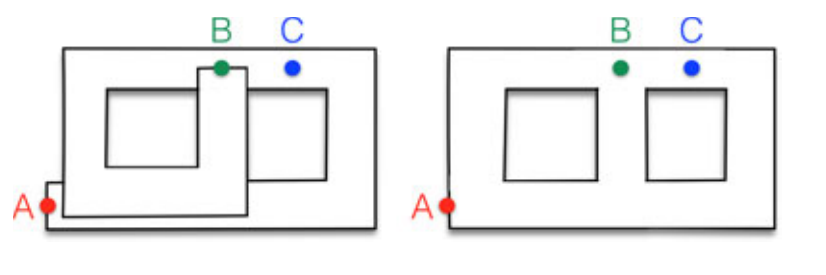
\includegraphics[scale=0.55]{Figures/infinite_corridor.png}
\centering
\caption{Left: a map built from odometry.It shows how the path from A to be is interpreted as a long corridor.Close points such as B and C may become arbitrarily far. Right: Map built using SLAM, where loop-closures allow the estimation of the true topology of the map. }
\label{figure:infinite_corridor}
\end{figure}

There are cases for SLAM algorithms can be considered largely solved  e.g. mapping an industrial environment using a robot equipped with wheel encoders and a two-dimensional range-finder (assumming sufficient accuracy and robustness). One example is \cite{roboticskuka}.
Other mature SLAM algorithm are Visual-based SLAM with slowly-moving robots (e.g. Mars rovers \cite{maimone2007two}, domestic robots \cite{ackerman2014dyson}) and visual-inertial odometry \cite{lynen2015get}.
\noindent However \cite{cadena2016past} states that all current SLAM algorithms could be induced to fail if the requirements on the robot motion or the structure of the environment are too challenging. E.g a visual SLAM algorithm could fail if it requires the robot to move quickly or an algorithm relying on a range-finder could fail in a fast-changing environment.
Although  states that there are SLAM algorithm.

\section{Literature Review Multi-Agent SLAM}
\label{section:litreview_slam}

-- TODO next semester --\\
-- distributed multi-robot slam --